\documentclass{beamer}

\definecolor{deepcarmine}{rgb}{0.66, 0.13, 0.24}
\usetheme{Madrid}
\usecolortheme[named=deepcarmine]{structure}
\usefonttheme[onlymath]{serif}
\usepackage{tikz}
\usetikzlibrary{shapes.geometric, arrows}


\title[Modelling Cholera Treatments]
{Examining Treatment Strategies for Cholera Incorporating Spatial Dynamics}
\author[Plague Doctors]{Group: Plague Doctors \\ Jessa Mallare, Sid Reed, Daniel Segura, Aref Jadda}
\institute[McMaster]{McMaster University \and
Instructor: Dr. David Earn}
\date[April 8, 2019]{April 8, 2019}

\tikzstyle{blocks} = [rectangle, draw, rounded corners, text width=3em, text centered, minimum height=3em, fill = green!30]
\tikzstyle{blocki} = [rectangle, draw, rounded corners, text width=3em, text centered, minimum height=3em, fill = red!30]
\tikzstyle{blockr} = [rectangle, draw, rounded corners, text width=3em, text centered, minimum height=3em, fill = yellow!30]
\tikzstyle{blockb} = [rectangle, draw, rounded corners, text width=3em, text centered, minimum height=3em, fill = blue!30]
\tikzstyle{blank} = [inner sep=0,outer sep=0]
\tikzstyle{line} = [draw,->,>=stealth]

\begin{document}

\begin{frame}
\titlepage
\end{frame}

\begin{frame}{Introduction}
\begin{itemize}
\setlength\itemsep{2em}
\item Treatments have not always gone as planned in history
\item Cholera
\end{itemize}
\end{frame}

\begin{frame}{Some Biology on Cholera}
\begin{itemize}
\setlength\itemsep{2em}
\item Vibrio cholerae
\item Colonize small intestines
\item 10% of infected develop symptoms
\item Causes dehydration
\end{itemize}
\end{frame}

\begin{frame}{Outbreaks in London ($19^{th}$ Century)}
\begin{columns}[onlytextwidth]
\column{0.5\textwidth}
\begin{itemize}
\setlength\itemsep{2em}
\item 1832, 1849, 1854, 1866
\item Miasma Theory
\item John Snow  
\end{itemize}
\column{0.5\textwidth}
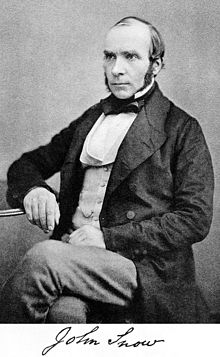
\includegraphics[width=0.65\textwidth]{Snow.jpg}
\end{columns}
\end{frame}

\begin{frame}{Single-Patch Model}
\begin{itemize}
\setlength\itemsep{2em}
\item Entire population (N) included
\item 3 Compartments : S, I, R
\item Compartment values are proportional
\item Environment (Water)
\end{itemize}
\end{frame}

\begin{frame}{SIRW Model Assumptions}
\begin{itemize}
\setlength\itemsep{2em}
\item Birth Rate = Natural Death Rate and is constant
\item Homogenous susceptibility to cholera across population
\item No waning immunity
\item No latency period
\item Only infected individuals can infect the water sources
\item Water source is still
\end{itemize}
\end{frame}

\begin{frame}{SIRW Model}
\begin{center}
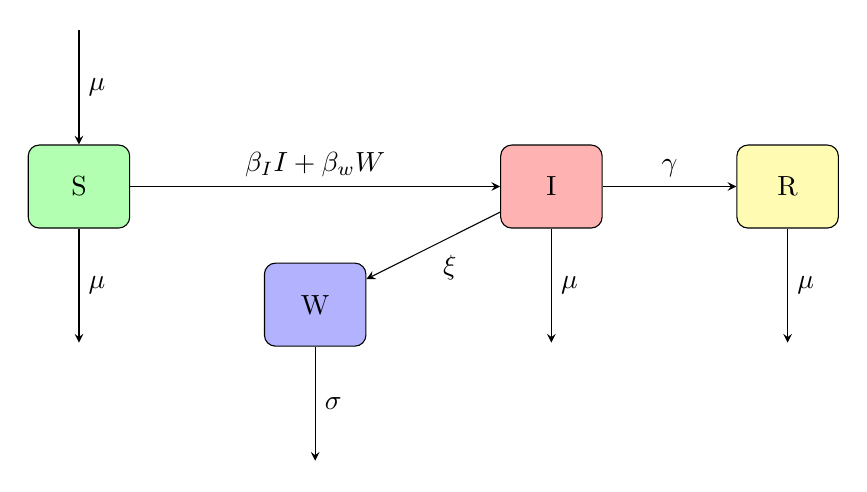
\begin{tikzpicture}[node distance=3cm, auto]

\node [blocks] (S) {S};
\node [blank, above of=S, yshift=-1cm] (0) { };
\node [blank, right of=S] (1) { };
\node [blockb, below of=1, yshift=1.5cm] (W) {W};
\node [blank, below of=W, yshift=1cm] (2) { };
\node [blocki, right of=1] (I) {I};
\node [blockr, right of=I] (R) {R};

\node [blank, below of=S, yshift=1cm] (3) {};
\node [blank, below of=I, yshift=1cm] (4) {};
\node [blank, below of=R, yshift=1cm] (5) {};

\path [line] (S) -- node {$\beta_I I + \beta_w W$} (I);
\path [line] (I) -- node {$\gamma$} (R);
\path [line] (I) -- node {$\xi$} (W);
\path [line] (W) -- node[anchor=west] {$\sigma$} (2);
\path [line] (0) -- node[anchor=west] {$\mu$} (S);

\path [line] (S) -- node[anchor=west] {$\mu$} (3);
\path [line] (I) -- node[anchor=west] {$\mu$} (4);
\path [line] (R) -- node[anchor=west] {$\mu$} (5);

\end{tikzpicture}
\end{center}
\end{frame}

\begin{frame}{SIWR Model Phase Portrait}

\end{frame}

\begin{frame}{$R_0$ Calculation}

\end{frame}

\begin{frame}{Equilibria and Stability}

\end{frame}

\begin{frame}{Final Size}

\end{frame}

\begin{frame}{Effect of the 19th Century Treatments}

\end{frame}

\begin{frame}{Multi-Patch Model}

\end{frame}

\begin{frame}{Multi-Patch Model Assumptions}
\begin{itemize}
\setlength\itemsep{2em}
\item No dispersal of individuals
\item Infected individuals can infect the susceptible in neighboring patches
\item All patches neighbouring i have the same transmission rate to patch i 
\end{itemize}
\end{frame}

\begin{frame}{Multi-Patch Model Simulation}

\end{frame}

\begin{frame}{Treatment Strategies For Cholera}
\begin{enumerate}
\setlength\itemsep{2em}
\item Sanitation of Water
\item Vaccinations
\item Antibiotics
\end{enumerate}
\end{frame}

\begin{frame}{Sanitation of Water}
\begin{center}
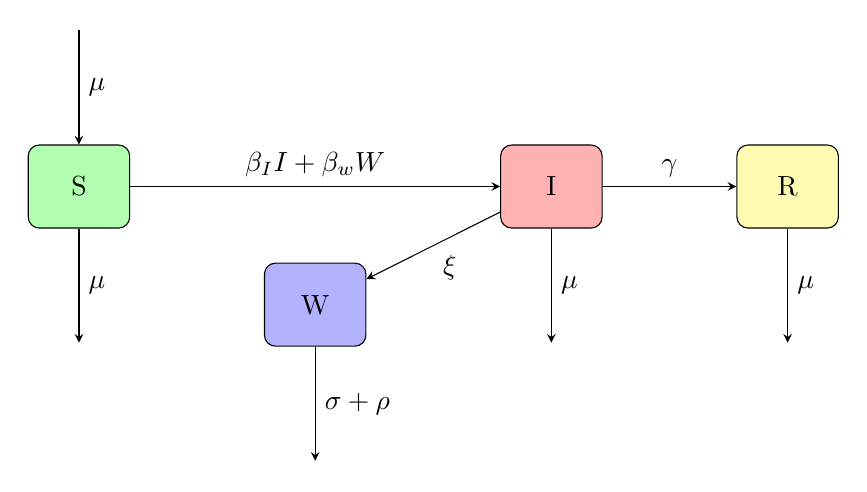
\begin{tikzpicture}[node distance=3cm, auto]

\node [blocks] (S) {S};
\node [blank, above of=S, yshift=-1cm] (0) { };
\node [blank, right of=S] (1) { };
\node [blockb, below of=1, yshift=1.5cm] (W) {W};
\node [blank, below of=W, yshift=1cm] (2) { };
\node [blocki, right of=1] (I) {I};
\node [blockr, right of=I] (R) {R};

\node [blank, below of=S, yshift=1cm] (3) {};
\node [blank, below of=I, yshift=1cm] (4) {};
\node [blank, below of=R, yshift=1cm] (5) {};

\path [line] (S) -- node {$\beta_I I + \beta_w W$} (I);
\path [line] (I) -- node {$\gamma$} (R);
\path [line] (I) -- node {$\xi$} (W);
\path [line] (W) -- node[anchor=west] {$\sigma + \rho$} (2);
\path [line] (0) -- node[anchor=west] {$\mu$} (S);

\path [line] (S) -- node[anchor=west] {$\mu$} (3);
\path [line] (I) -- node[anchor=west] {$\mu$} (4);
\path [line] (R) -- node[anchor=west] {$\mu$} (5);

\end{tikzpicture}
\end{center}
\end{frame}

\begin{frame}{Vaccinations}
\begin{center}
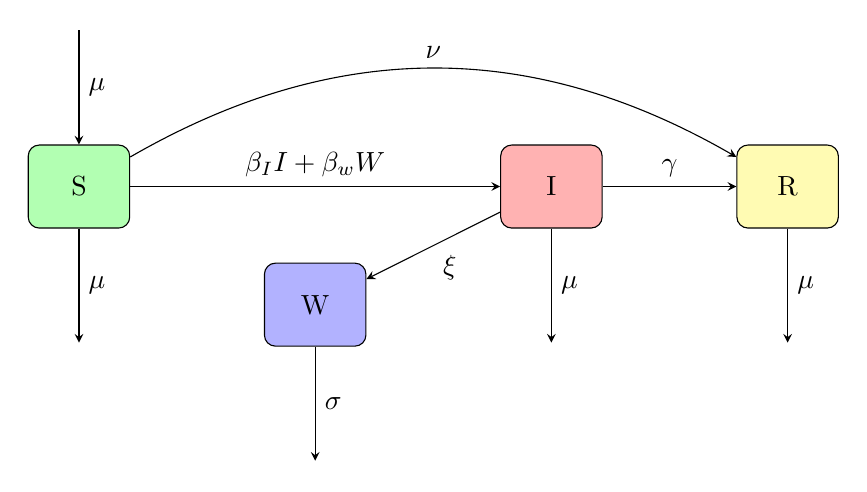
\begin{tikzpicture}[node distance=3cm, auto]

\node [blocks] (S) {S};
\node [blank, above of=S, yshift=-1cm] (0) { };
\node [blank, right of=S] (1) { };
\node [blockb, below of=1, yshift=1.5cm] (W) {W};
\node [blank, below of=W, yshift=1cm] (2) { };
\node [blocki, right of=1] (I) {I};
\node [blockr, right of=I] (R) {R};

\node [blank, below of=S, yshift=1cm] (3) {};
\node [blank, below of=I, yshift=1cm] (4) {};
\node [blank, below of=R, yshift=1cm] (5) {};

\path [line] (S) -- node {$\beta_I I + \beta_w W$} (I);
\path [line] (S) to [bend left,looseness=1] node[above] {$\nu$} (R);
\path [line] (I) -- node {$\gamma$} (R);
\path [line] (I) -- node {$\xi$} (W);
\path [line] (W) -- node[anchor=west] {$\sigma$} (2);
\path [line] (0) -- node[anchor=west] {$\mu$} (S);

\path [line] (S) -- node[anchor=west] {$\mu$} (3);
\path [line] (I) -- node[anchor=west] {$\mu$} (4);
\path [line] (R) -- node[anchor=west] {$\mu$} (5);

\end{tikzpicture}
\end{center}
\end{frame}

\begin{frame}{Antibiotics}
\begin{center}
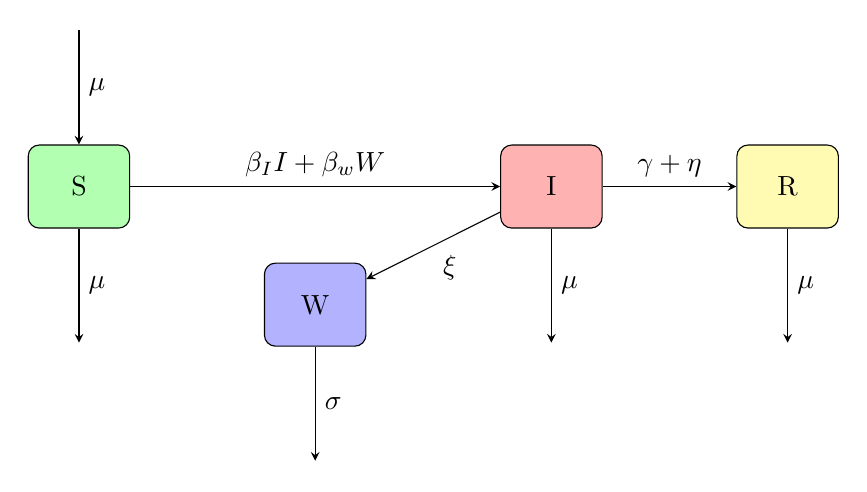
\begin{tikzpicture}[node distance=3cm, auto]

\node [blocks] (S) {S};
\node [blank, above of=S, yshift=-1cm] (0) { };
\node [blank, right of=S] (1) { };
\node [blockb, below of=1, yshift=1.5cm] (W) {W};
\node [blank, below of=W, yshift=1cm] (2) { };
\node [blocki, right of=1] (I) {I};
\node [blockr, right of=I] (R) {R};

\node [blank, below of=S, yshift=1cm] (3) {};
\node [blank, below of=I, yshift=1cm] (4) {};
\node [blank, below of=R, yshift=1cm] (5) {};

\path [line] (S) -- node {$\beta_I I + \beta_w W$} (I);
\path [line] (I) -- node {$\gamma + \eta$} (R);
\path [line] (I) -- node {$\xi$} (W);
\path [line] (W) -- node[anchor=west] {$\sigma$} (2);
\path [line] (0) -- node[anchor=west] {$\mu$} (S);

\path [line] (S) -- node[anchor=west] {$\mu$} (3);
\path [line] (I) -- node[anchor=west] {$\mu$} (4);
\path [line] (R) -- node[anchor=west] {$\mu$} (5);

\end{tikzpicture}
\end{center}
\end{frame}

\begin{frame}{Comparing the Treatment Strategies}

\end{frame}

\begin{frame}{Comparing the Treatment Strategies}

\end{frame}

\begin{frame}{Conclusions and Further Research}
\begin{itemize}
\setlength\itemsep{2em}
\item 19th century outbreaks
\item Significance of the using multi-patch model
\item Our treatment simulations suggest…
\item Further research on the spread of water borne diseases like cholera can be done in areas like…
\end{itemize}
\end{frame}

\begin{frame}
\begin{center}
{\huge Thank you!}
\end{center}
\end{frame}



\end{document}
